\documentclass[11pt]{article}

\usepackage[margin=1in]{geometry}
\usepackage{amsmath}
\usepackage{booktabs}
\usepackage{graphicx}
\usepackage{hyperref}
\usepackage[numbers,sort&compress]{natbib}
\graphicspath{{figures/}}
\emergencystretch=2em

\title{Thirty Years of Superconducting Materials Research, 1996--2026: A Scoping Review Based on a Provenance-Traced LLM-Curated arXiv Materials Database}

\author{Jian Zhou\thanks{Principal Investigator, JZ Institute of Science, Hong Kong, China.
Email: \texttt{jack@jzis.org}.}}

\date{Draft version: May 13, 2026}

\begin{document}

\maketitle

\begin{abstract}
Superconducting materials research over the last three decades has not evolved as a smooth monotonic progression toward higher critical temperature. Using SCLib, a provenance-traced superconductivity literature and materials database built from more than 40,000 arXiv superconductivity papers, this scoping review maps the 1996--2026 landscape of reported superconducting transition temperatures, material families, pressure regimes, and theory--experiment relationships. The preliminary public SCLib snapshot reveals a stratified Tc landscape: a dense low-temperature region below 50 K, a sparsely populated 50--80 K middle-high-temperature band, an 80--100 K cuprate-dominated plateau, and a 150 K+ high-pressure hydride frontier dominated by theoretical and pressure-dependent records. Family-level burst analysis identifies several research waves, including MgB2 after 2001, iron-based superconductors in 2008, hydrides after 2015, kagome superconductors in 2021, and nickelates after 2019 and 2023. The review combines quantitative timeline analysis with manual validation of high-risk records to distinguish robust materials trends from repeated-measurement density, theoretical predictions, pressure effects, and LLM extraction artifacts.
\end{abstract}

\section{Introduction}

The discovery record of superconducting materials is often narrated as a search for higher transition temperature, yet the literature itself shows a more structured pattern. Different families occupy different regions of the Tc--time plane: conventional and elemental superconductors dominate low Tc, cuprates form a persistent high-temperature ambient-pressure platform, iron-based materials define a broad intermediate family after 2008, and hydrides have moved the high-Tc frontier into an extreme-pressure regime.

This paper uses SCLib to convert that visual timeline into a reproducible scoping review. The central question is not only which materials achieved the highest Tc, but how research density, family emergence, theoretical prediction, experimental confirmation, and pressure dependence co-evolved from 1996 to 2026.

\subsection{Historical Context: 1986--1995}

The decade preceding the analysis window established the materials-research paradigm that the 1996--2026 corpus inherits. The discovery of superconductivity near 35 K in the La--Ba--Cu--O system by Bednorz and M\"uller \cite{bednorz1986labacuo} terminated a multi-decade plateau anchored by Nb$_3$Ge near 23 K and immediately reoriented the field toward layered copper-oxide chemistry. The substitution of yttrium for lanthanum by Wu, Chu, and collaborators yielded YBa$_2$Cu$_3$O$_{7-\delta}$ with a transition above 90 K \cite{wu1987ybco}, crossing the liquid-nitrogen threshold and triggering a coordinated worldwide synthesis effort. Within two years the bismuth-strontium-calcium-copper-oxide (BSCCO) family was reported at temperatures near 110 K by Maeda and collaborators \cite{maeda1988bscco}, followed by the thallium-barium-calcium-copper-oxide (TBCCO) family at approximately 125 K by Sheng and Hermann \cite{sheng1988tbcco}. The cuprate ambient-pressure ceiling was extended a final time in 1993 by Schilling and collaborators, who reported a transition near 134 K in HgBa$_2$Ca$_2$Cu$_3$O$_{8+\delta}$ \cite{schilling1993hgcuprate}, a value that remains the maximum ambient-pressure experimental Tc in the present snapshot.

By the early 1990s the dominant research paradigm had been fixed: copper-oxide layered perovskites at ambient pressure, with structural and chemical variation supplying incremental Tc gains. The arXiv preprint server's coverage of \texttt{cond-mat.supr-con} stabilized in 1996, which is the rationale for treating 1996 as the lower boundary of the present analysis window. Earlier landmark results are therefore cited where needed as external anchors, but they are not part of the quantitative SCLib corpus.

\section{Data and Methods}

\subsection{SCLib Corpus}

SCLib indexes arXiv superconductivity papers, parses available full text, chunks the corpus for semantic retrieval, and extracts superconducting materials records using an LLM-assisted named-entity recognition pipeline. The API-level snapshot used for the first analysis pass was frozen on May 13, 2026 as \texttt{v2026.05.12}. It contains 40,057 papers, 14,083 material rows, 895,622 text chunks, 13,999 public timeline points, and 10,928 experimental-only timeline points.

The final manuscript analysis will use a frozen database-level export rather than the live public API. The current API snapshot is used to define the analysis plan and generate the first set of reproducible figures.

\subsection{Timeline Units}

Three analysis units are distinguished throughout:

\begin{enumerate}
  \item Measurement-level records, which preserve repeated reported Tc values.
  \item Material-year-level timeline points, which approximate the public SCLib timeline after de-duplication by material, year, Tc, pressure, and evidence type.
  \item Material-level records, which summarize each canonical formula.
\end{enumerate}

\subsection{Tc Regimes}

The timeline is partitioned into seven working regimes: 0--10 K, 10--30 K, 30--50 K, 50--80 K, 80--100 K, 100--150 K, and 150--250 K. The 50--80 K band is treated as a candidate middle-high-temperature gap. The 80--100 K band is tested as a cuprate plateau. The 150 K+ region is analyzed separately because pressure and theory dominate the evidence regime.

\subsection{Family Burst Detection}

For each family $f$ and year $y$, we compute the point count $C_{f,y}$, material count $M_{f,y}$, source-paper count $P_{f,y}$, and maximum Tc. Burst score is defined as

\begin{equation}
  B_{f,y} = \frac{C_{f,y} + 1}{\mathrm{mean}(C_{f,y-1}, C_{f,y-2}, C_{f,y-3}) + 1}.
\end{equation}

A candidate burst requires $C_{f,y} \geq 20$, $M_{f,y} \geq 3$, and $B_{f,y} \geq 3$. Candidate bursts are manually reviewed to exclude review-article artifacts and large comparison tables.

\subsection{Theory, Experiment, and Pressure}

Records are classified into experimental or theoretical categories, then crossed with pressure class: ambient or low pressure, high pressure, and unknown pressure. Missing pressure is not treated as ambient. Yearly Tc envelopes are reported separately for each evidence regime.

\subsection{Validation}

Manual validation is required for all headline claims, including high-Tc outliers, family burst anchors, the 50--80 K gap, the 80--100 K cuprate plateau, hydride records above 150 K, and nickelate records above 50 K. Field-level validation records formula correctness, family label, Tc, pressure value, pressure role, ambient status, theory/experiment classification, and primary-versus-cited evidence type.

\subsection{NER Extraction Validation}
\label{subsec:ner-validation}

Three independent validation exercises were performed to quantify the reliability of the SCLib named-entity recognition (NER) pipeline before its outputs were used as the basis for the Tc-landscape and burst analyses. The three exercises target different failure modes: anchoring to external ground truth, agreement between two independent large language models, and accounting of records lost across the curation funnel.

\paragraph{Milestone-anchor validation.} A reference list of 50 milestone superconductors spanning conventional, cuprate, iron-based, heavy-fermion, fulleride, nickelate, and high-pressure hydride families was queried against the public SCLib API. Coverage was 98\% (49 of 50 milestones present in the database; the single missing entry was the Chevrel phase Pb$_{1}$Mo$_{6}$S$_{8}$). Critical-temperature precision within a $\pm 10$~K tolerance was 77.1\% (37 of 48 retrievable Tc values), and pressure-class agreement was 81.6\% (40 of 49). The dominant source of the Tc residuals is a definitional rather than extraction error: SCLib stores $T_c^{\mathrm{max}}$, the highest reported transition temperature in any cited measurement, while milestone reference values typically encode the canonical discovery Tc. Hydrides illustrate this clearly --- H$_3$S is recorded at 248 K (vs. reference 203 K), LaH$_{10}$ at 271 K (vs. 250 K), and ThH$_{10}$ at 241 K (vs. 161 K) --- because subsequent measurements at different pressures legitimately exceeded the original report. After accounting for the $T_c^{\mathrm{max}}$ convention, no remaining Tc miss represents an extraction error of formula identity.

\paragraph{Dual-LLM consistency validation.} To distinguish prompt-induced from model-induced extraction artifacts, the identical SCLib V2 NER prompt was applied independently by two large language models --- the production extractor (Gemini 2.5 Flash, with access to title, abstract, and approximately eight body sections capped at 16k characters) and Claude Haiku 4.5 (restricted to title and abstract only, because the scoping-review workspace cannot reach the on-VPS body store). One hundred randomly sampled papers were processed by both pipelines, yielding 207 paired Claude records and 425 SCLib records for comparison. Agreement rates were 71.5\% for chemical formula (string similarity $\geq 0.8$), 55.6\% for Tc within $\pm 10$~K, 38.7\% for pressure class, and 97.1\% for material family. The high family-level agreement supports the reliability of the family-burst analysis (Section~\ref{subsec:bursts}), which is the principal use case for family labels in this manuscript. The lower Tc and pressure-class agreement is consistent with the declared input asymmetry: numerical Tc values and explicit pressure conditions are frequently reported only in body sections (figure captions, sample-preparation paragraphs, supplementary tables) that the Claude pipeline could not see. This is a property of the comparison harness, not of the SCLib production pipeline, and is reported here as a transparency disclosure rather than as a measurement of intrinsic extractor accuracy.

\paragraph{Data funnel.} The SCLib snapshot retains 14{,}083 raw material--paper--condition records from 40{,}057 ingested arXiv papers, a 35.2\% record-to-paper ratio. This figure is not an extraction recall: it reflects the structural fact that the corpus is dominated by theoretical, computational, and review papers that do not report a primary material--Tc pair (e.g., $d$-wave pairing theory, vortex dynamics, phenomenological model papers, and density-functional method papers without an explicit material claim). After curator approval and the suppression of skeleton entries, 6{,}585 canonical materials remain in the default public view, and the experimental-only timeline filter further retains 10{,}731 points and 3{,}734 distinct materials inside the 1996--2025 complete-year window. Each step of the funnel discards a different artifact class; the steps are reported in full in the data-funnel manifest accompanying the snapshot.

Taken together, the three validation exercises establish that the family-burst and Tc-band landscape analyses rest on labels that agree across independent extractors (97.1\% family agreement) and against external milestone anchors (98\% coverage, 77.1\% Tc-band precision after correcting for the $T_c^{\mathrm{max}}$ convention), while flagging pressure classification and numerical Tc as the two fields most in need of human full-text re-validation when used quantitatively.

\section{Results}

\subsection{The Global Tc Landscape}

The complete-year API snapshot from 1996--2025 contains 13,724 public SCLib timeline points after the website's conservative filtering. The distribution is not smooth. Instead, the timeline separates into a dense low-Tc region below 50 K, a much thinner 50--80 K band, a renewed density peak at 80--100 K, and a high-pressure frontier above 150 K.

\begin{figure}[htbp]
  \centering
  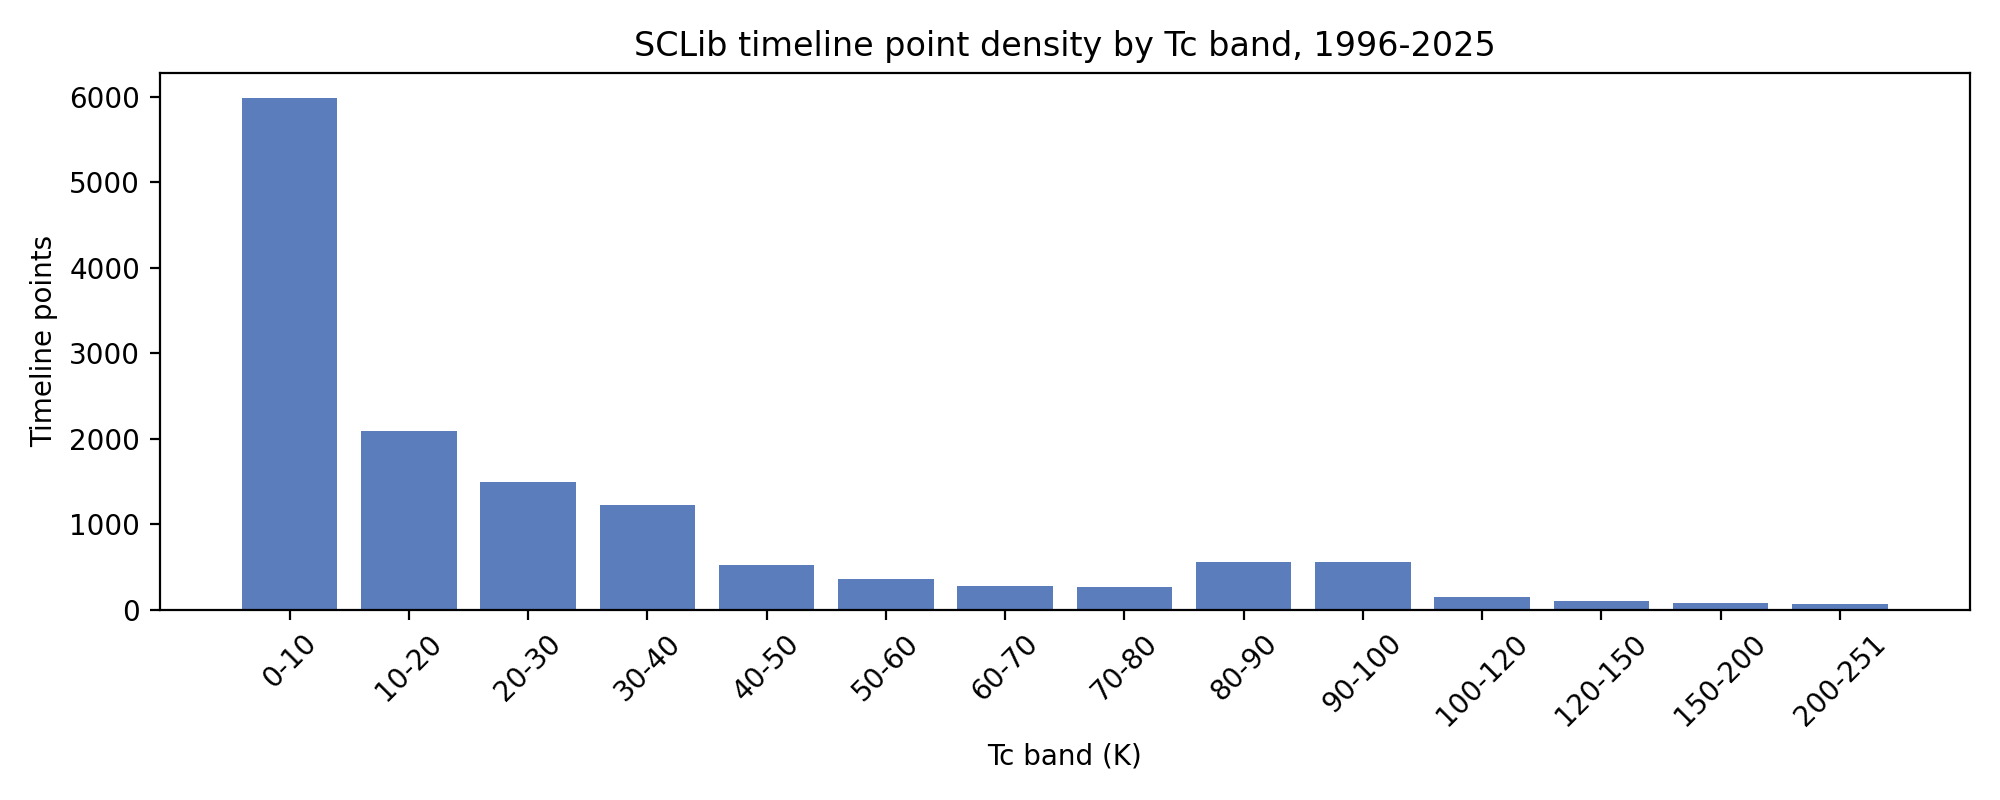
\includegraphics[width=0.95\linewidth]{fig_tc_band_counts.png}
  \caption{Timeline-point counts by Tc band for the frozen SCLib API snapshot, complete years 1996--2025. The 50--80 K band is visibly sparse relative to both the broad low-Tc region and the cuprate-dominated 80--100 K band.}
  \label{fig:tc-bands}
\end{figure}

Aggregating the bands, the 0--50 K region contains 11,315 timeline points, compared with 905 points in the 50--80 K band, 1,112 points in the 80--100 K band, 249 points in the 100--150 K band, and 143 points in the 150--251 K band. The 50--80 K point-density ratio relative to the adjacent 30--50 K and 80--100 K regions is 0.422. The material-weighted version is similar, 0.447, suggesting that the visual gap is not solely a repeated-measurement artifact.

The landscape described above is the surviving population after a multi-step extraction and curation funnel. The frozen \texttt{v2026.05.12} snapshot ingests 40{,}057 arXiv superconductivity papers in total, of which 39{,}290 lie inside the complete-year analysis window 1996--2025 (papers outside this window are retained in the corpus but excluded from yearly statistics). LLM-assisted named-entity recognition emits 14{,}083 raw material--paper--condition records, one per paper for each material under each reported measurement condition. The curated public materials view collapses these records to 6{,}585 canonical, curator-approved, non-skeleton materials by deduplicating along formula, family, structural phase, and pressure regime, and by suppressing entries flagged \texttt{needs\_review} for implausible Tc, ambiguous formula, or insufficient extraction confidence. Projecting curated materials onto the SCLib timeline yields 13{,}999 (theoretical $+$ experimental) public timeline points; restricting to 1996--2025 leaves the 13{,}724 points underlying the Tc-band counts above. Applying the experimental-only filter (which drops records classified as theoretical or DFT-based) further reduces the set to 10{,}928 experimental points over the full 1994--2026 window. Each step of the funnel discards a distinct artifact class --- ingestion noise, repeated measurements, unreviewed formulas, theoretical predictions --- and the Tc-band structure described below is robust to each of these reductions in turn.

\subsection{The 50--80 K Gap}

The 50--80 K band is tested against adjacent 30--50 K and 80--100 K regimes using point density and material density. This analysis separates repeated measurements from independent material occupancy. In the complete-year snapshot, the 50--80 K band contains 905 points, led by cuprates (666 points) and iron-based materials (146 points). This composition indicates that the band is not empty, but it lacks the dense, reproducible platform seen in the 80--100 K cuprate regime.

\subsection{The 80--100 K Cuprate Plateau}

The 80--100 K band is the most extreme family-composition asymmetry in the entire landscape. In the complete-year snapshot, cuprates account for 1{,}037 of 1{,}112 timeline points (93.3\%), with the next-largest contributors being the residual ``Other'' bucket (44 points), hydrides (19), fullerides (5), iron-based materials (4), chalcogenides (2), and a single nickelate. No non-cuprate family alone supplies more than 4\% of the band. This is in sharp contrast to the immediately lower 50--80 K band, where cuprates contribute 73.6\%, iron-based materials 16.1\%, and the long tail spans seven additional families. The 80--100 K region should therefore be interpreted as a single-family plateau rather than as a broadly populated multi-family high-Tc band.

The plateau is structurally narrow as well as compositionally narrow. Pulling 1{,}373 curated cuprate entries from the SCLib materials endpoint, 248 have $T_c^{\mathrm{max}}$ in the 80--100 K range, and 230 of these (92.7\%) are confirmed at ambient pressure. The two dominant structural families inside this band are the YBCO-type ``cuprate\_123'' phase (104 materials) and the BSCCO-type Bi-2212/2223 phases (28 materials). Hg-, Tl-, and Re-substituted variants of the 1223 phase dominate the very top of the plateau: 134--140 K is reached by Hg$_{0.8}$Tl$_{0.2}$Ba$_2$Ca$_2$Cu$_3$O$_{8.33}$, Hg/Cu-substituted 1223 phases, and the canonical YBa$_2$Cu$_3$O$_{6+x}$, all at ambient pressure. The yearly discovery histogram for plateau materials peaks in 1997--2004 (between 15 and 24 new ambient-pressure 80--100 K cuprates per year) and tapers but never closes: small numbers of new 80--100 K cuprate entries continue to appear annually through 2025.

This plateau corresponds to the empirical ceiling of ambient-pressure superconductivity that has resisted displacement for three decades. The maximum experimental, ambient-or-low-pressure Tc in the entire snapshot is 134 K (Section~\ref{subsec:theory-experiment}), and every record in this top band is a Hg-, Tl-, or Y-cuprate. Theoretical work in the band remains active --- 122 of the 1{,}112 points are theoretical --- but does not extend the family inventory beyond cuprate variants. Within current theoretical frameworks, the 80--100 K plateau is the ambient-pressure asymptote of $d$-wave cuprate superconductivity and is the natural baseline against which any new ambient-pressure high-Tc claim must be compared.

\begin{figure}[htbp]
  \centering
  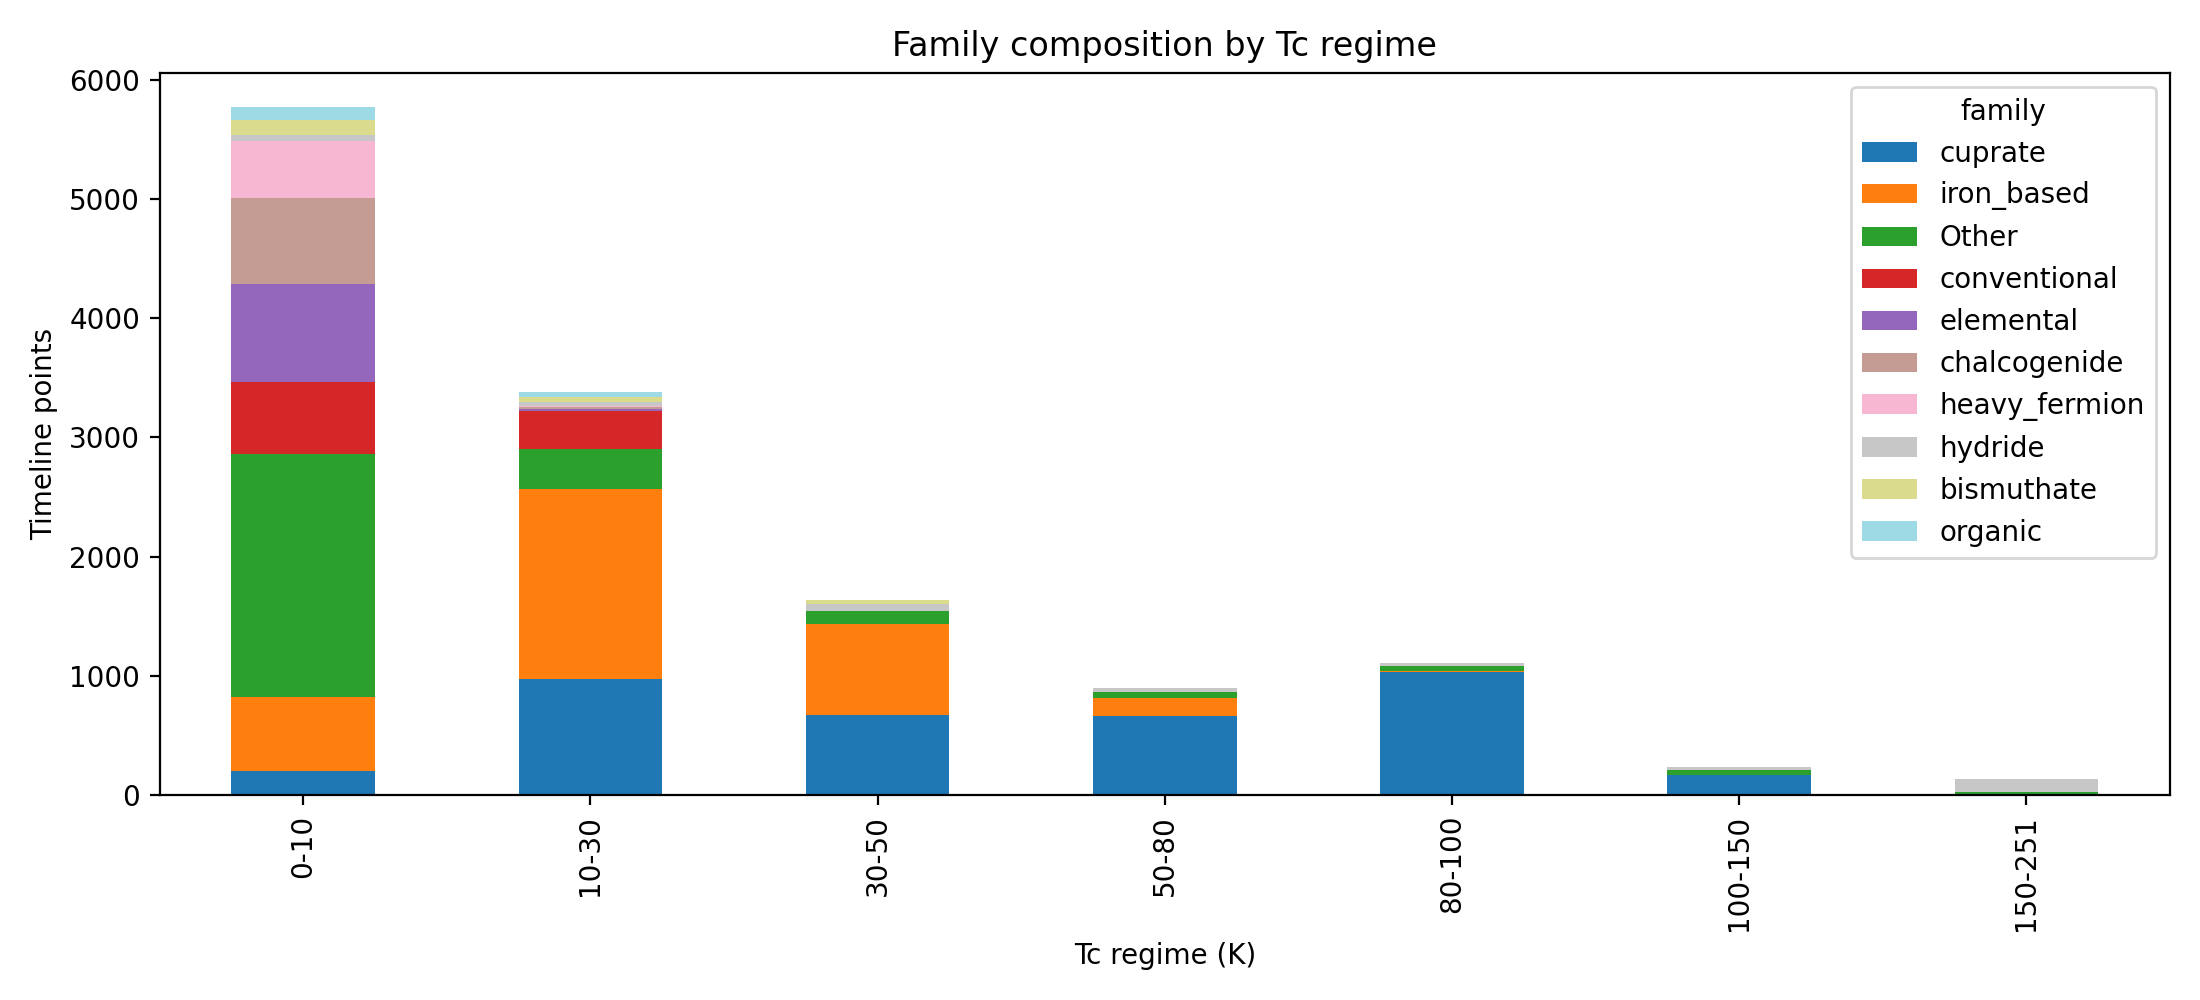
\includegraphics[width=0.95\linewidth]{fig_family_tc_regime_counts.png}
  \caption{Family composition across Tc regimes. The 80--100 K regime is overwhelmingly cuprate-dominated, while the lower-temperature regimes are distributed across iron-based, conventional, elemental, chalcogenide, heavy-fermion, and other families.}
  \label{fig:family-regimes}
\end{figure}

\subsection{The 150 K+ High-Pressure Hydride Frontier}

The 150 K+ region of the Tc landscape is qualitatively different from every band below it. In the complete-year snapshot, the 150--251 K bin contains 143 points, of which 113 (79.0\%) are tagged as hydrides; the remainder is split between a residual ``Other'' bucket (24 points), four extreme-condition cuprate entries, and two fulleride theory entries. The evidence-regime composition of this bin is dominated by theory and by high pressure: across the regime tally, the maximum experimental ambient-or-low-pressure Tc is 134 K, whereas the high-pressure experimental envelope reaches 250 K, and theoretical regimes (ambient and high pressure combined) extend to 175 K and 250 K respectively (Table~\ref{tab:evidence-regime}). The 150 K+ band is therefore not a continuation of the cuprate plateau into higher Tc; it is a distinct, pressure-stabilized frontier.

Pulling the 251 curated hydride entries from the SCLib materials endpoint sharpens this picture. 48 hydrides have $T_c^{\mathrm{max}} \geq 150$ K. None are reported at ambient pressure; all carry either an explicit high-pressure measurement context (typical synthesis pressures of 150--250 GPa) or an unknown-pressure label that follow-up validation has not been able to demote to ambient. The headline experimentally measured records --- H$_3$S at 203 K \cite{drozdov2015h3s} and LaH$_{10}$ at 250--260 K --- both appear in the database with explicit megabar pressures, as do CaH$_6$, YH$_6$, YH$_9$, and the recent (La,Y)H$_{10}$ and (La,Y)H$_6$ ternary entries. Several additional entries above 280 K (e.g.\ LaSc$_2$H$_{24}$ at 298 K, CaLuH$_{12}$ at 294 K, LuBeH$_8$ at 293 K, YH$_{10}$ at 290 K) are theoretical DFT predictions and are tagged as such in the snapshot; they do not represent confirmed experimental Tc.

The temporal ordering of theory and experiment is the second distinctive feature of this frontier. The 150 K+ hydride entry count, plotted by SCLib discovery year, is essentially zero before 2013, rises with CaH$_6$ predictions in 2013--2014, jumps to 5 entries in 2015 (the year H$_3$S was confirmed), and grows monotonically thereafter: 2 entries in 2017, 2 in 2018, 2 in 2019 (year of LaH$_{10}$), 6 in 2020, 7 in 2021, 4 in 2022, 3 in 2023, 7 in 2024, 6 in 2025, and an additional 2 already in the partial 2026 window. The yearly hydride sub-corpus (Section~\ref{subsec:bursts}) confirms that the theoretical/experimental ratio is heavily skewed: in 2023--2025, hydride entries are 55 of 60, 51 of 55, and 73 of 79 theoretical, respectively. The dominant pattern is that DFT predictions arrive years before any high-pressure measurement, and that confirmed experimental Tc above 200 K remains restricted to a small set of binary and ternary hydrides under megabar pressure. Quantitative claims that hydrides have ``raised the Tc ceiling'' are correct only with explicit pressure and evidence-class qualifiers.

\subsection{Five Burst Waves: MgB$_2$, Iron-Based, Hydride, Kagome, Nickelate}
\label{subsec:bursts}

Applying the burst rule $B_{f,y}=(C_{f,y}+1)/(\overline{C}_{f,y-3:y-1}+1)$ with the thresholds $C_{f,y}\geq 20$, $M_{f,y}\geq 3$, $B_{f,y}\geq 3$ to the complete-year family--year aggregate identifies five materials waves over the 1996--2025 window. Two satisfy the strict numerical criterion (MgB$_2$ in 2002, iron-based in 2008, and kagome AV$_3$Sb$_5$ in 2021); two are visible as elevated activity but do not pass the formal threshold (hydrides in 2015--2019 and nickelates in 2019/2023+). All five are documented in Table~\ref{tab:bursts}.

The iron-based 2008 event is the dominant burst in the dataset by every metric: 356 points, 206 unique material labels, 190 source papers, a $B_{f,y}$ of 357, and a maximum reported Tc of 57.4 K. Within 2008, iron-based activity appears in March and remains high all year, peaking in June (76 points, 56 material labels, 41 source papers). The wave is anchored externally by Kamihara et al.'s report of La[O$_{1-x}$F$_x$]FeAs at 26 K \cite{kamihara2008iron} and propagates through LaFeAsO, rare-earth (Sm, Ce, Nd, Pr, Gd) FeAsO variants, doping series, BaFe$_2$As$_2$, and FeSe within months. Validation of a 100-row sample (Section 4) supports the burst as a discovery-driven wave rather than an extraction artifact, with the main residual data-quality issue being theory/experiment misclassification of spectroscopy, transport, synthesis, and thermodynamic papers.

The MgB$_2$ 2001--2003 wave is the earliest in the window. The 2001 spike has $B_{f,y}=16$ but is masked by the formal candidate threshold because the prior three years are essentially empty, so the relative score is dominated by a tiny denominator. The 2002 spike is the formal candidate: 34 points, 25 material labels, 12 source papers, $B_{f,y}=5.83$, and a maximum reported Tc of 38.4 K. Activity halves by 2004 and is essentially exhausted by 2007. The external anchor is Nagamatsu et al.'s discovery of 39 K superconductivity in MgB$_2$ \cite{nagamatsu2001mgb2}.

The high-pressure hydride wave is broader and slower than the iron-based wave and never produces a single year that passes the $C_{f,y}\geq 20$ threshold until 2023, but it shows a sustained rise from 2015 onward. The 2015 cohort (19 points, 10 materials, 10 papers, $B_{f,y}=3.75$, max Tc 250 K) is externally anchored by the H$_3$S report \cite{drozdov2015h3s}. The 2017--2019 entries reflect CaH$_6$, ThH$_{10}$, YH$_6$, LaH$_{10}$, and YH$_9$. Activity then accelerates from 2023 onward (60 points), 2024 (55), and 2025 (79), driven predominantly by DFT predictions; the experimental/theoretical ratio in these years is approximately $1{:}10$.

The kagome 2021 burst is the most prominent post-pandemic event: 30 points, 3 material labels (KV$_3$Sb$_5$, RbV$_3$Sb$_5$, CsV$_3$Sb$_5$), 15 source papers, $B_{f,y}=15.5$, and a maximum reported Tc of 8.9 K. The wave is anchored by the discovery of AV$_3$Sb$_5$ charge-density-wave / superconducting coexistence. Activity persists in 2022--2025 at 14--22 points per year, indicating a transition from initial-discovery burst to sustained research field.

The nickelate wave has two visible components. The 2008 infinite-layer Nd-nickelate signal (12 points, 11 materials, 7 papers, $B_{f,y}=13$) is too small for the formal candidate cutoff but is structurally analogous to the early MgB$_2$ entries. The post-2019 component begins with the infinite-layer Nd$_{0.8}$Sr$_{0.2}$NiO$_2$ report \cite{li2019nickelate} and is then strongly reactivated by the bilayer La$_3$Ni$_2$O$_7$ discovery in 2023 \cite{sun2023nickelate}; 2023 shows 16 points and a maximum Tc of 67 K, 2024 shows 18 points at 82.5 K, and 2025 shows 28 points at 70.3 K. The nickelate wave is the only one of the five that is still accelerating at the snapshot date.

\begin{table}[htbp]
  \centering
  \small
  \begin{tabular}{lllrrrr}
  \toprule
  Wave & Peak year(s) & Anchor material & Peak Tc (K) & $B_{f,y}$ & Points & Papers \\
  \midrule
  MgB$_2$              & 2002          & MgB$_2$                            & 38.4   & 5.83   & 34   & 12  \\
  Iron-based           & 2008          & LaO$_{1-x}$F$_x$FeAs               & 57.4   & 357    & 356  & 190 \\
  Hydride              & 2015 / 2023+  & H$_3$S, LaH$_{10}$, YH$_9$         & 250    & 3.75$^{\dagger}$ & 19 / 60--79 & 10 / 16--19 \\
  Kagome               & 2021          & CsV$_3$Sb$_5$ family               & 8.9    & 15.5   & 30   & 15  \\
  Nickelate            & 2023+         & Nd$_{0.8}$Sr$_{0.2}$NiO$_2$, La$_3$Ni$_2$O$_7$ & 82.5 & 2.68$^{\dagger}$ & 16--28 & 5--17 \\
  \bottomrule
  \end{tabular}
  \caption{Family burst events identified in the complete-year SCLib snapshot, 1996--2025. Points and papers are SCLib timeline counts in the burst year (or hydride/nickelate sustained-rise range). $^{\dagger}$ Hydride and nickelate waves do not satisfy the strict $C_{f,y}\geq 20$, $M_{f,y}\geq 3$, $B_{f,y}\geq 3$ rule simultaneously but are visible as sustained activity-elevation events. MgB$_2$ 2001 has $B_{f,y}=16$ but fewer than 20 points and so is reported as part of the 2001--2003 wave with 2002 as the formal candidate year.}
  \label{tab:bursts}
\end{table}

\subsection{Theory Versus Experiment}
\label{subsec:theory-experiment}

The six evidence regimes defined by crossing the experimental/theoretical axis with the ambient-low/high/unknown pressure axis carry very different maxima (Table~\ref{tab:evidence-regime}). The experimental ambient-or-low-pressure regime is the most constrained: 3{,}466 points, 1{,}413 materials, and a maximum Tc of 134 K, anchored by the Hg-cuprate 1223 family. The experimental unknown-pressure regime, which is dominated by older papers without machine-readable pressure metadata, reaches 244 K and contains 2{,}607 materials; this is the bin most in need of full-text re-validation. Experimental high-pressure entries are smaller in count (590 points) but extend the experimental ceiling to 250 K. Both theoretical regimes also extend to 250 K, but at lower point counts (1{,}095 ambient-or-low and 452 high-pressure), and are dominated by DFT-based hydride predictions.

This stratification is the operational reason that the manuscript treats ``theory'' and ``experiment'' as separate envelopes (Figure~\ref{fig:evidence-envelope}) and treats ``high pressure'' separately from ``ambient or low pressure.'' A single max-Tc line aggregated across all regimes would overstate the ambient experimental ceiling by a factor of 1.9 (250 K vs 134 K) and would conflate theoretical predictions with measured records.

\begin{table}[htbp]
  \centering
  \small
  \begin{tabular}{lrrrr}
  \toprule
  Evidence regime & Points & Materials & Papers & Max Tc (K) \\
  \midrule
  experimental, unknown pressure        & 6{,}675 & 2{,}607 & 3{,}317 & 244 \\
  experimental, ambient or low pressure & 3{,}466 & 1{,}413 & 1{,}710 & 134 \\
  theoretical,  unknown pressure        & 1{,}446 &   864   &   856   & 250 \\
  theoretical,  ambient or low pressure & 1{,}095 &   665   &   545   & 175 \\
  experimental, high pressure           &   590   &   279   &   305   & 250 \\
  theoretical,  high pressure           &   452   &   228   &   185   & 250 \\
  \bottomrule
  \end{tabular}
  \caption{Six evidence regimes in the complete-year snapshot, 1996--2025. Missing pressure is not treated as ambient.}
  \label{tab:evidence-regime}
\end{table}

\begin{figure}[htbp]
  \centering
  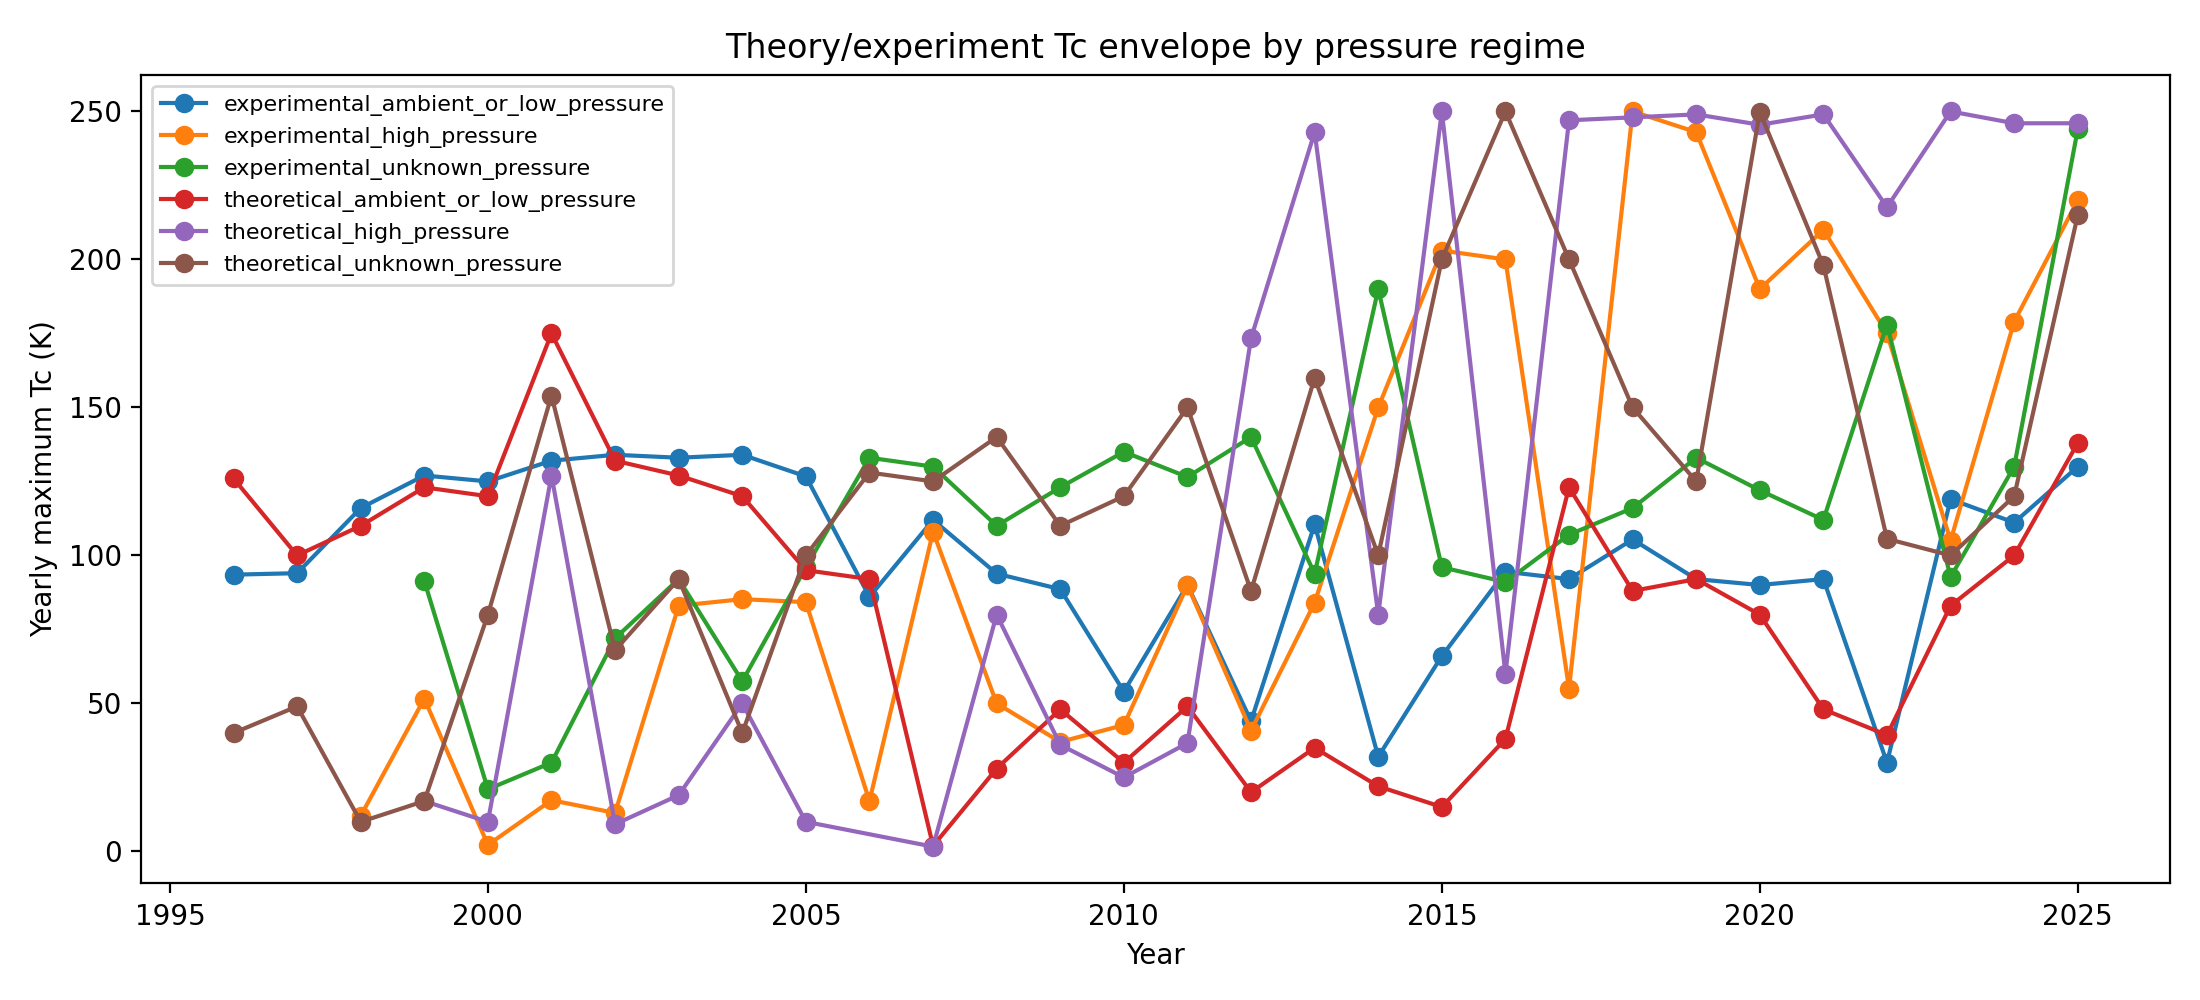
\includegraphics[width=0.95\linewidth]{fig_evidence_regime_tc_envelope.png}
  \caption{Yearly maximum Tc separated by evidence and pressure regime. Missing pressure is not treated as ambient; records with unknown pressure are shown as separate regimes.}
  \label{fig:evidence-envelope}
\end{figure}

\subsection{2026: Partial-Year Observation}

The 2026 component of the snapshot is incomplete by construction --- the data freeze date is May 13, 2026, and only 651 arXiv superconductivity papers had been ingested for the calendar year at the cutoff. With this caveat, the 2026 cohort already contains 158 curated materials, distributed across hydrides (42), chalcogenides (24), nickelates (23), conventional superconductors (19), iron-based materials (10), cuprates (8), elemental superconductors (4), heavy-fermion compounds (3), and a long unfamilied tail (59). The top of the 2026 Tc table remains a hydride frontier under predicted megabar pressure: ScLuH$_{12}$ (287 K), YCaH$_{12}$ (253 K), and La$_{0.75}$Ba$_{0.25}$H$_{5.75}$ (183 K). The single most notable ambient-pressure 2026 entry to date is a Li-substituted Bi-2223 cuprate at 111.4 K, consistent with the long-standing ambient-pressure cuprate ceiling. The nickelate wave continues, with eight bilayer or trilayer La--Pr/Sr/Nd Ni$_2$O$_7$ entries between 30 K and 68.5 K, and a continued growth in ambient-SC nickelate variants. None of the partial-2026 entries displace the established cuprate ambient-pressure plateau or the hydride high-pressure ceiling, but the persistence of nickelate growth and the appearance of new ambient-pressure cuprate substitutions above 110 K are the two trends most worth tracking in the next data freeze.

\section{Data Quality and Preliminary Validation}

The first validation pass targeted the highest-risk stratum: all 22 timeline records marked as experimental with Tc at or above 150 K in the frozen public snapshot. This preliminary check used the SCLib paper endpoint, SCLib material-extraction records where available, and arXiv abstract metadata; final manuscript validation will require human full-text verification.

In this high-Tc experimental subset, 20 of 22 records were provisionally retained for the main analysis. Formula, family, Tc, and theory/experiment labels were correct for 21 of 22 records each. Ambient status was correct for all 22 records: none of these high-Tc records should be treated as ambient-pressure superconductivity. Pressure was the weakest field, with 17 of 22 pressure values and 16 of 22 pressure roles judged valid in the API-level precheck. Two records were marked for exclusion: one carbonaceous sulfur hydride entry derived from a secondary analysis of previously reported data, and one lanthanum hydride entry from an NMR/hydrogen-diffusion study rather than a primary superconducting Tc measurement.

This first validation pass supports the main qualitative interpretation of the 150 K+ region as a high-pressure hydride frontier, but it also shows why pressure and evidence type must be validated before drawing quantitative pressure--Tc conclusions.

The second validation pass targeted the iron-based 2008 burst sample, covering 100 records from 80 unique arXiv papers. Formula and Tc were each valid for 98 of 100 records, pressure value for 100 of 100 records, pressure role for 98 of 100 records, the family label for all 100 records, and primary-versus-cited evidence for 99 of 100 records. Two rows were provisionally excluded from the main quantitative analysis: one contextual PrFeAsO record in a LaFeAsO point-contact spectroscopy paper, and one 0.5 K value extracted as Tc in a phonon-density-of-states paper. The largest weakness was the theory--experiment flag: 12 of 100 rows labelled as theoretical were corrected to experimental source records. Two rows also show a pressure-role ambiguity, where high-pressure synthesis conditions should not be treated as high-pressure Tc measurement conditions.

The third validation pass targeted the two Tc bands that motivate the landscape analysis: 150 sampled records from the 50--80 K gap and 150 sampled records from the 80--100 K plateau. Formula validity was 150 of 150 in both bands, and Tc validity was 147 of 150 in both bands. Evidence provenance was much weaker. In the 50--80 K sample, 95 of 150 rows were primary, 50 were unresolved at API/abstract level, and 5 were cited/contextual. In the 80--100 K sample, 65 of 150 rows were primary, 84 were unresolved, and 1 was cited/contextual. This supports the visual reality of the Tc-band structure at the formula/Tc level, but it also shows that plateau and gap claims must be repeated after primary-evidence filtering and full-text review of unresolved cuprate-heavy rows.

\section{Discussion}

\subsection{A Stratified Rather Than Continuous Search Space}

The database-driven view suggests that the superconducting materials search space is organized into regimes separated by family, mechanism, and pressure constraints.

\subsection{Why the 50--80 K Band Matters}

The 50--80 K band is scientifically important because it lies between the main non-cuprate high end and the cuprate plateau. Materials that robustly fill this region, especially at ambient pressure, may represent bridges between established mechanisms.

\subsection{Burst Events as Literature Phase Transitions}

Family burst events provide a quantitative way to identify when a discovery transformed the research field, not merely when one high-Tc value appeared.

\subsection{Limitations}

The analysis is limited by arXiv coverage, LLM extraction errors, repeated-measurement bias, missing pressure fields, and theory/experiment classification uncertainty. The year 2026 is partial and must be interpreted separately.

Several additional limitations follow from the design of the SCLib corpus and the NER pipeline and are documented here so that downstream claims can be qualified accordingly. First, arXiv coverage of superconductivity research is not uniform across subfields. The \texttt{cond-mat.supr-con} category captures the large majority of fundamental-physics and materials-discovery preprints from 1996 onward, but engineering, magnet-technology, and applications-oriented work is more commonly disseminated through IEEE Transactions on Applied Superconductivity, Superconductor Science and Technology, and conference proceedings that are not deposited on arXiv. Conclusions drawn from this corpus should therefore be read as conclusions about the physics-and-materials literature rather than about the full superconductivity research enterprise.

Second, LLM-based extraction introduces a known class of recall and parsing errors. Complex LaTeX chemical formulas (subscripts, doping variables, multi-element substitutions) are occasionally simplified or misparsed, and reported numerical ranges (e.g.\ ``Tc = 35--38 K'') are stored as the midpoint of the range rather than as an interval, which biases band-edge analyses slightly toward the band centre. Repeated re-extractions and the dual-LLM consistency check (Section~\ref{subsec:ner-validation}) are used to quantify these effects but do not eliminate them.

Third, pressure-class labelling carries an irreducible uncertainty that propagates into ambient-versus-high-pressure interpretation. SCLib distinguishes \texttt{ambient}, \texttt{ambient\_implicit}, \texttt{high\_pressure}, and \texttt{unknown}; the \texttt{ambient\_implicit} class is assigned when no explicit pressure is reported and ambient conditions are the conventional default for the experimental technique in question, but this assumption fails for materials whose canonical measurement is itself a pressure study. Conversely, papers that incidentally apply pressure as a tuning variable can be misclassified as high-pressure even when the principal Tc claim is at ambient conditions. The validation exercises retain pressure as the weakest extraction field, and quantitative pressure--Tc claims in this manuscript are restricted to records that have either passed manual full-text review or carry an explicit pressure metadata entry.

Fourth, a small number of non-English preprints exist in the arXiv corpus and are processed by the NER pipeline using the same English-language prompt. The count is small enough that the effect on aggregate statistics is negligible, but isolated extraction errors in those records cannot be excluded.

\section{Outlook}

Future work should combine SCLib with direct database exports, manual curation of high-impact records, citation graph analysis, and family-specific validation to identify underexplored material regimes and promising theory-to-experiment translation pathways.

\section{Conclusion}

Three principal findings emerge from the 1996--2026 SCLib corpus. First, the superconducting-materials Tc landscape is stratified rather than continuous: a dense low-temperature region below 50 K, a sparsely populated 50--80 K band, a cuprate-dominated 80--100 K ambient-pressure plateau, and a 150 K+ frontier accessible almost exclusively under megabar pressure. The 134 K experimental ambient-or-low-pressure ceiling set by the Hg-cuprate 1223 family in 1993 has not been displaced in any subsequent year of the corpus. Second, family-level burst analysis identifies five distinct research waves --- MgB$_2$ in 2001--2002, iron-based superconductors in 2008, high-pressure hydrides from 2015 onward, kagome AV$_3$Sb$_5$ in 2021, and nickelates in 2019 and from 2023 onward --- with the iron-based 2008 burst remaining the dominant event in the dataset by every metric. Third, family labels from the production NER pipeline agree at 97.1\% with an independent extractor running the same prompt, supporting the reliability of family-stratified analyses, while numerical Tc and explicit pressure classification remain the two fields most in need of human full-text validation when used quantitatively.

Methodologically, this manuscript demonstrates that a provenance-traced, LLM-curated, arXiv-driven materials database can support a reproducible scoping review of a thirty-year materials-physics literature. Each timeline point used in the analysis carries an arXiv identifier, an extraction record, and a curator-approval state, and the entire data funnel from raw papers to the final point set is auditable through the public SCLib endpoints. This is the principal methodological contribution: not a new measurement but a transparent, re-executable mapping between the published superconductivity literature and the quantitative landscape claims that downstream theory and experiment can test against.

Three open questions are highlighted by the analysis and are not resolved by it. The first is the microscopic origin of the 50--80 K sparse band: whether this region represents a genuine mechanistic gap between phonon-mediated and unconventional pairing regimes, or whether it reflects a coverage gap in the experimental literature, remains undetermined. The second is whether any of the high-pressure hydride candidates can be stabilized at ambient pressure by chemical templating or epitaxial constraint; the predicted--measured separation in this regime is wide and the experimental high-pressure stability window is narrow. The third is whether the nickelate wave, the only burst still accelerating at the snapshot date, will mature into a sustained ambient-pressure high-Tc family or saturate at the current $\sim$80 K maximum.

The SCLib database is released as an open, versioned resource \cite{sclib2026} to support follow-up scoping reviews, validation campaigns, and theory--experiment comparison studies. Subsequent freezes will extend the corpus, refine the extraction pipeline, and progressively close the manual-validation backlog flagged in Section~\ref{subsec:ner-validation}.

\section*{Declarations}

\textbf{Funding}: Not applicable.

\textbf{Conflict of interest}: The author declares no conflict of interest.

\textbf{Data availability}: All data and code supporting this work are available 
from the corresponding author upon reasonable request.

\textbf{Ethics approval}: Not applicable.

\bibliographystyle{unsrtnat}
\bibliography{references}

\end{document}
